\chapter{Testing}\label{ch:testing}

This chapter of the report will detail the testing conducted on the configured AWS services.
This was done to determine the accuracy and efficiency of the configurations made during the deployment process.
The testing was conducted by using Gherkin, a language used to define behaviour and test
cases~\parencite{dos2018automated}.
It is non-technical and is intended to be easily human-readable.
Gherkin uses set keywords for structure and meaning: Given, When, and Then.
An example of this structure can be seen in Figure~\ref{fig:gherkin}.

\begin{figure}[!htbp]
    \centering
    \begin{minted}{cucumber}
    Scenario: Does the web application work?
        Given ...
        When ...
        Then ...
    \end{minted}
    \label{fig:gherkin}
\end{figure}

EC2, S3, CloudFront, RDS, CloudWatch, and CloudTrail were all tested using this approach.
Screenshots are included to illustrate the results of these tests.

\section{Testing EC2}\label{sec:testing-ec2}

\begin{figure}[!htbp]
    \centering
    \begin{minted}{cucumber}
Scenario: Accessing instance through SSH with .pem file private key.
    Given that the EC2 instance is running on AWS and the user has EC2 keypair
    When the user enters the command
    "ssh -i Group4_KeyPair.pem ec2-user@52.45.13.111" in the terminal
    Then the user will be logged into the EC2 instance
    \end{minted}
    \label{fig:accessing-instance-ec2}
\end{figure}

\begin{figure}[!htbp]
    \centering
    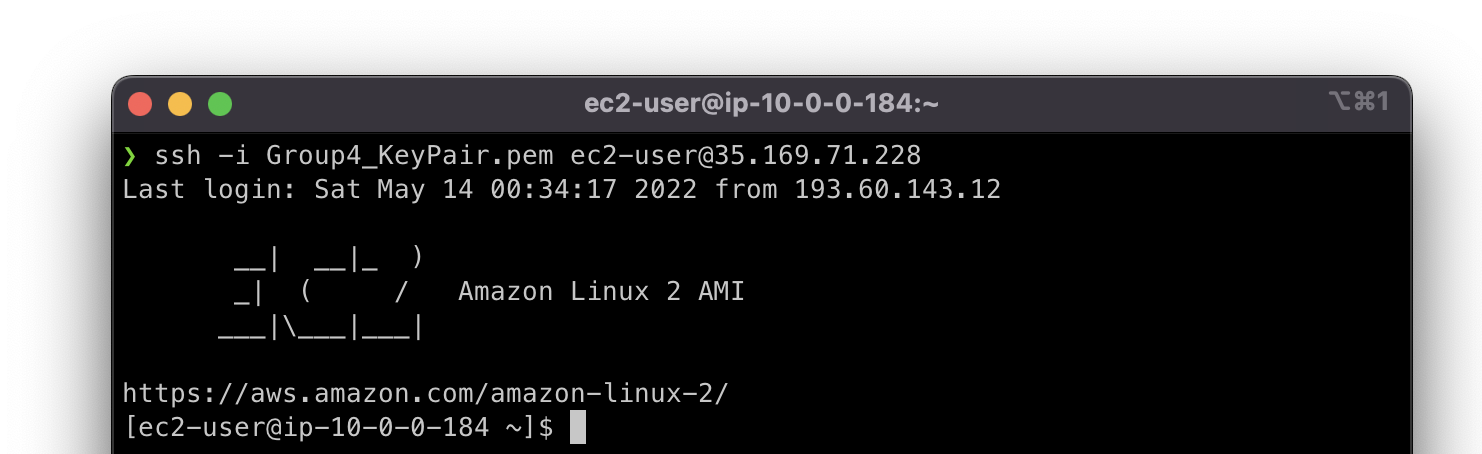
\includegraphics[width=\textwidth]{resources/ec2/ec2-logged-in}
    \label{fig:ec2-test-logged-in}
\end{figure}

\clearpage

\begin{figure}[!htbp]
    \centering
    \begin{minted}{cucumber}
Scenario: Accessing web app through EC2 domain name.
    Given that the web app is running on the EC2 instance
    When the user accesses
    "http://ec2-52-45-13-111.compute-1.amazonaws.com" in their browser
    Then the web app will be loaded
    \end{minted}
    \label{fig:accessing-web-app-ec2}
\end{figure}

\begin{figure}[!htbp]
    \centering
    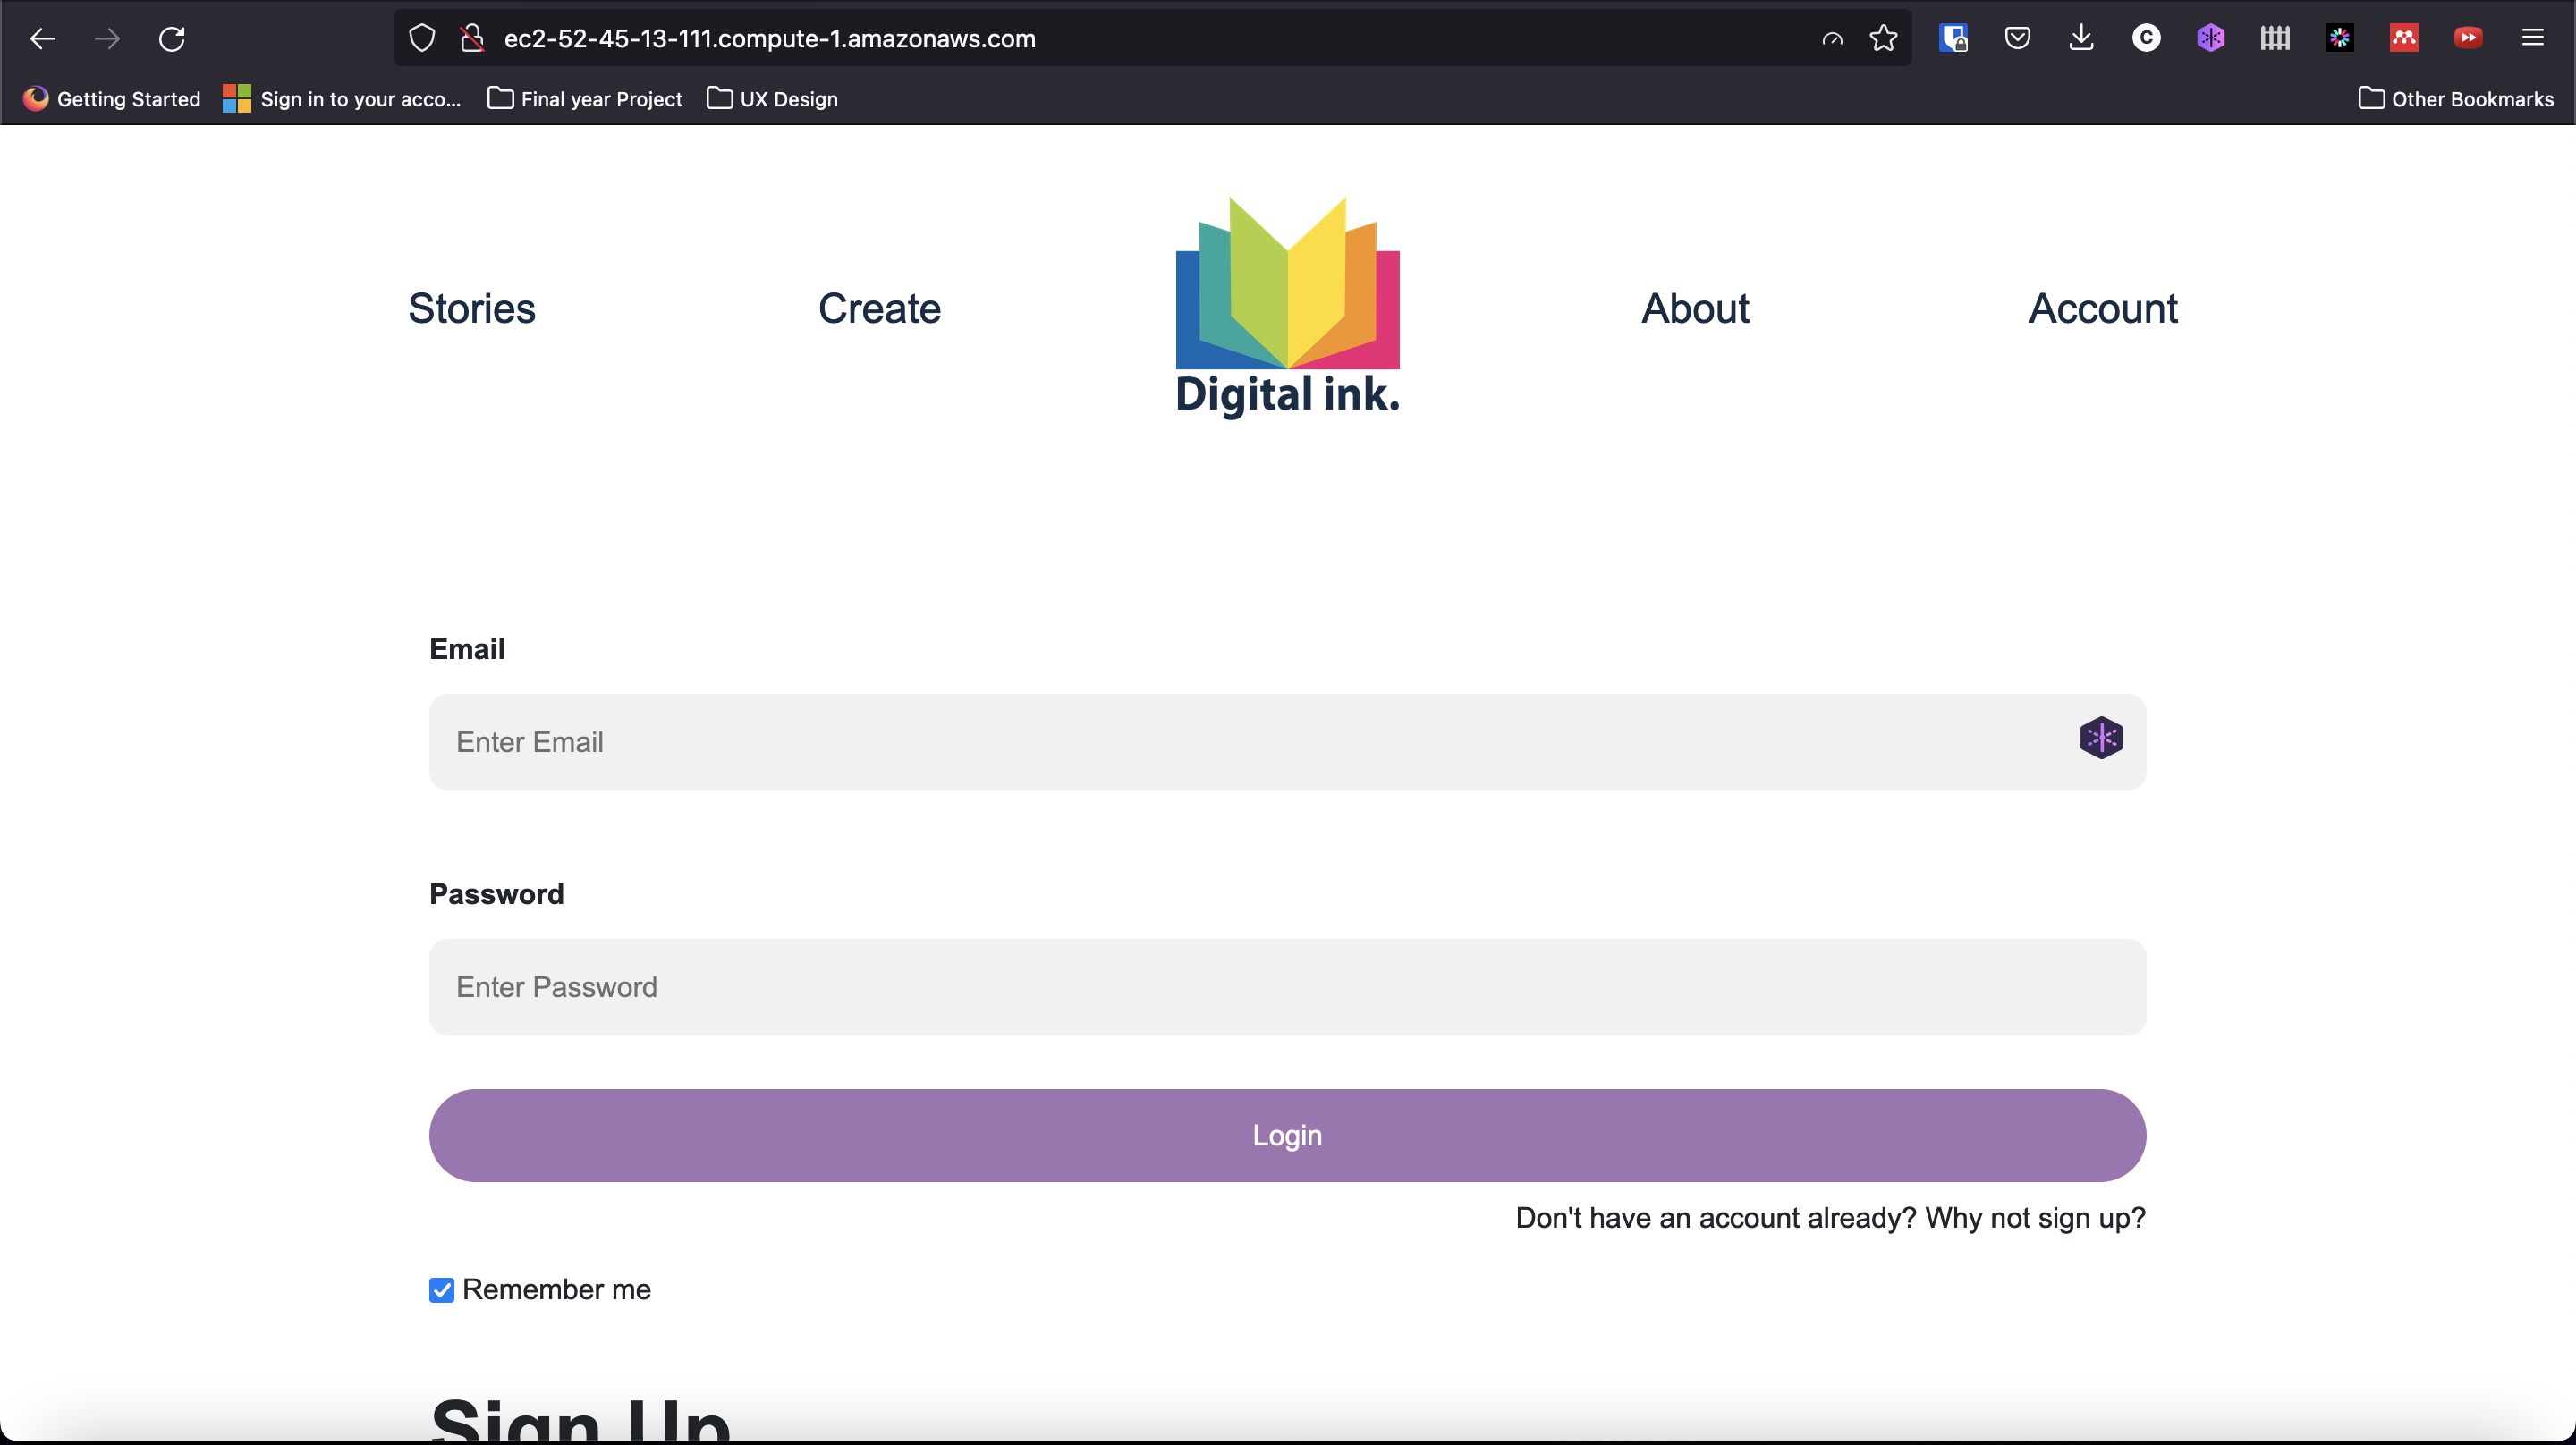
\includegraphics[width=\textwidth]{resources/ec2/digital-ink-ec2}
    \label{fig:ec2-test-digital-ink}
\end{figure}

\clearpage

\section{Testing S3}\label{sec:testing-s3}

\begin{figure}[!htbp]
    \centering
    \begin{minted}{cucumber}
Scenario: Accessing web app image through S3 domain name.
    Given that an image on the web app is in an S3 bucket
    When the user accesses the URL
    "https://group4-digital-ink-s3.s3.amazonaws.com/" followed by the name of the image
    Then the user will see the image displayed from the S3 bucket
    \end{minted}
    \label{fig:accessing-image-s3}
\end{figure}

\begin{figure}[!htbp]
    \centering
    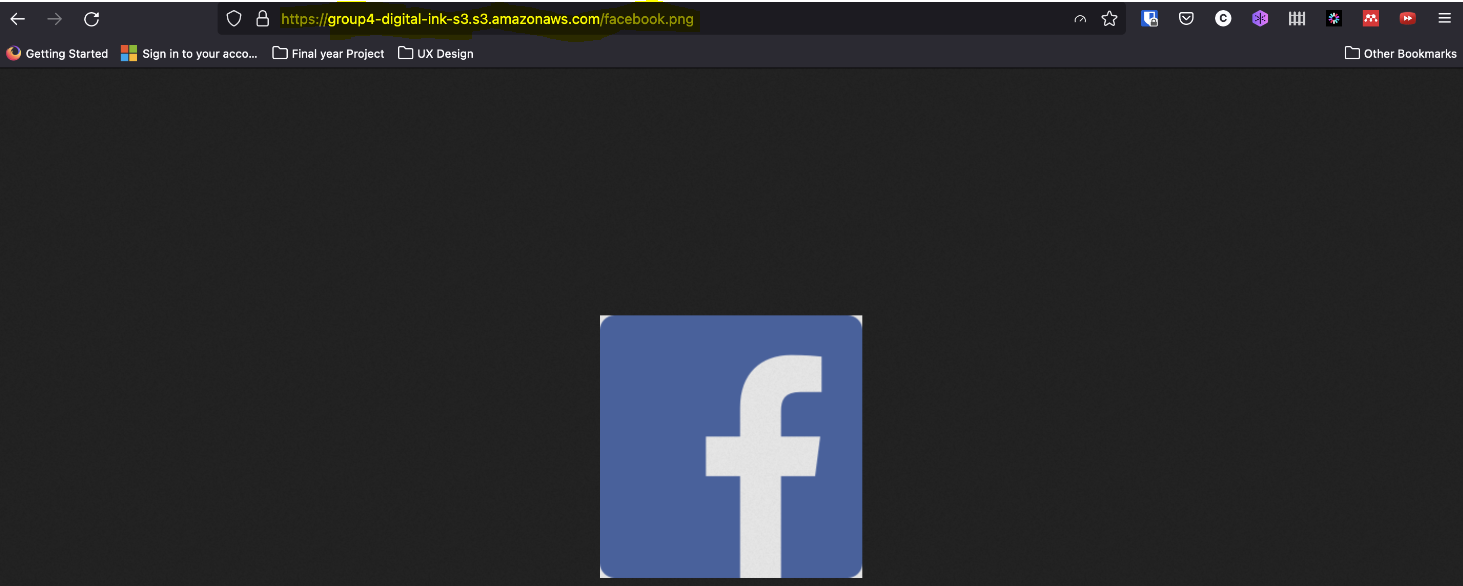
\includegraphics[width=\textwidth]{resources/s3/s3-image-displayed}
    \label{fig:s3-test-photo}
\end{figure}

\clearpage

\section{Testing CloudFront}\label{sec:testing-cloudfront}

\begin{figure}[!htbp]
    \centering
    \begin{minted}{cucumber}
Scenario: Accessing web app image through CloudFront domain name.
    Given that an image on the web app is in a CloudFront distribution
    When the user accesses the URL
    "https://d1bdkf7iuqj4qy.cloudfront.net/" followed by the name of the image
    Then the user will see the image displayed from the CloudFront distribution
    \end{minted}
    \label{fig:accessing-image-cloudfront}
\end{figure}

\begin{figure}[!htbp]
    \centering
    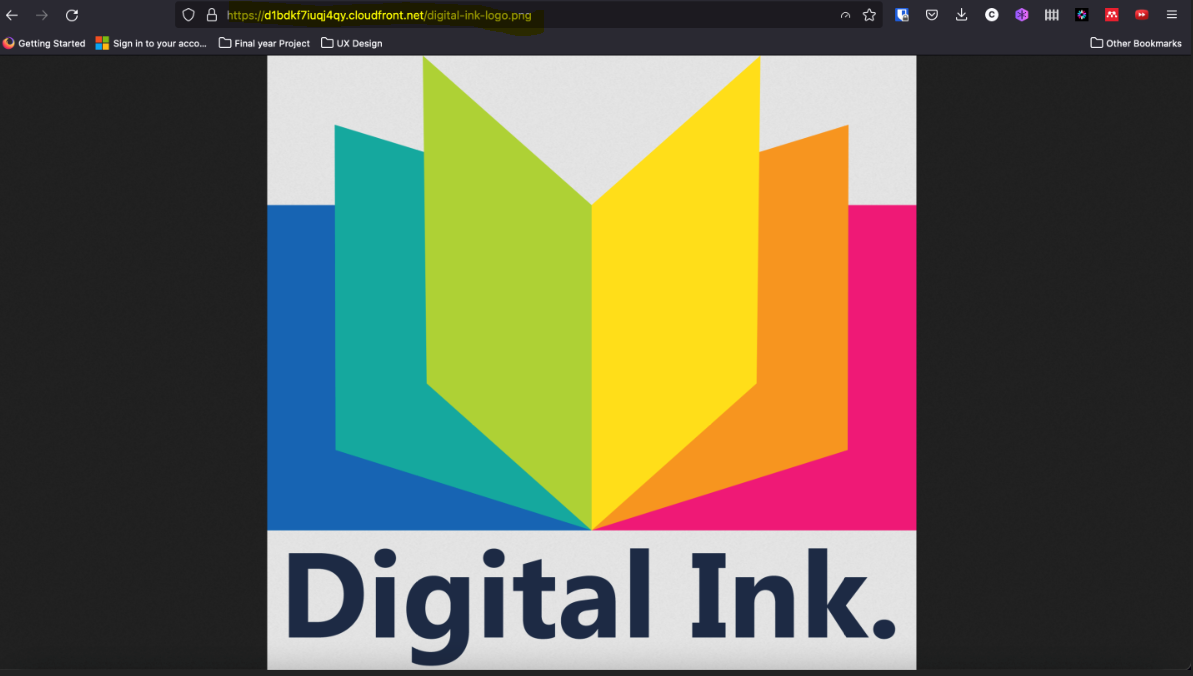
\includegraphics[width=\textwidth]{resources/cloudfront/cloudfront-website}
    \label{fig:cloudfront-test-photo}
\end{figure}

\clearpage

\begin{figure}[!htbp]
    \centering
    \begin{minted}{cucumber}
Scenario: Accessing web app image through CloudFront domain name in another region.
    Given that the user is connected to the internet
    When the user accesses a resource on the web app
    Then CloudFront will distribute that content in the region closest to them
    \end{minted}
    \label{fig:accessing-image-cloudfront-diff-region}
\end{figure}

\begin{figure}[!htbp]
    \centering
    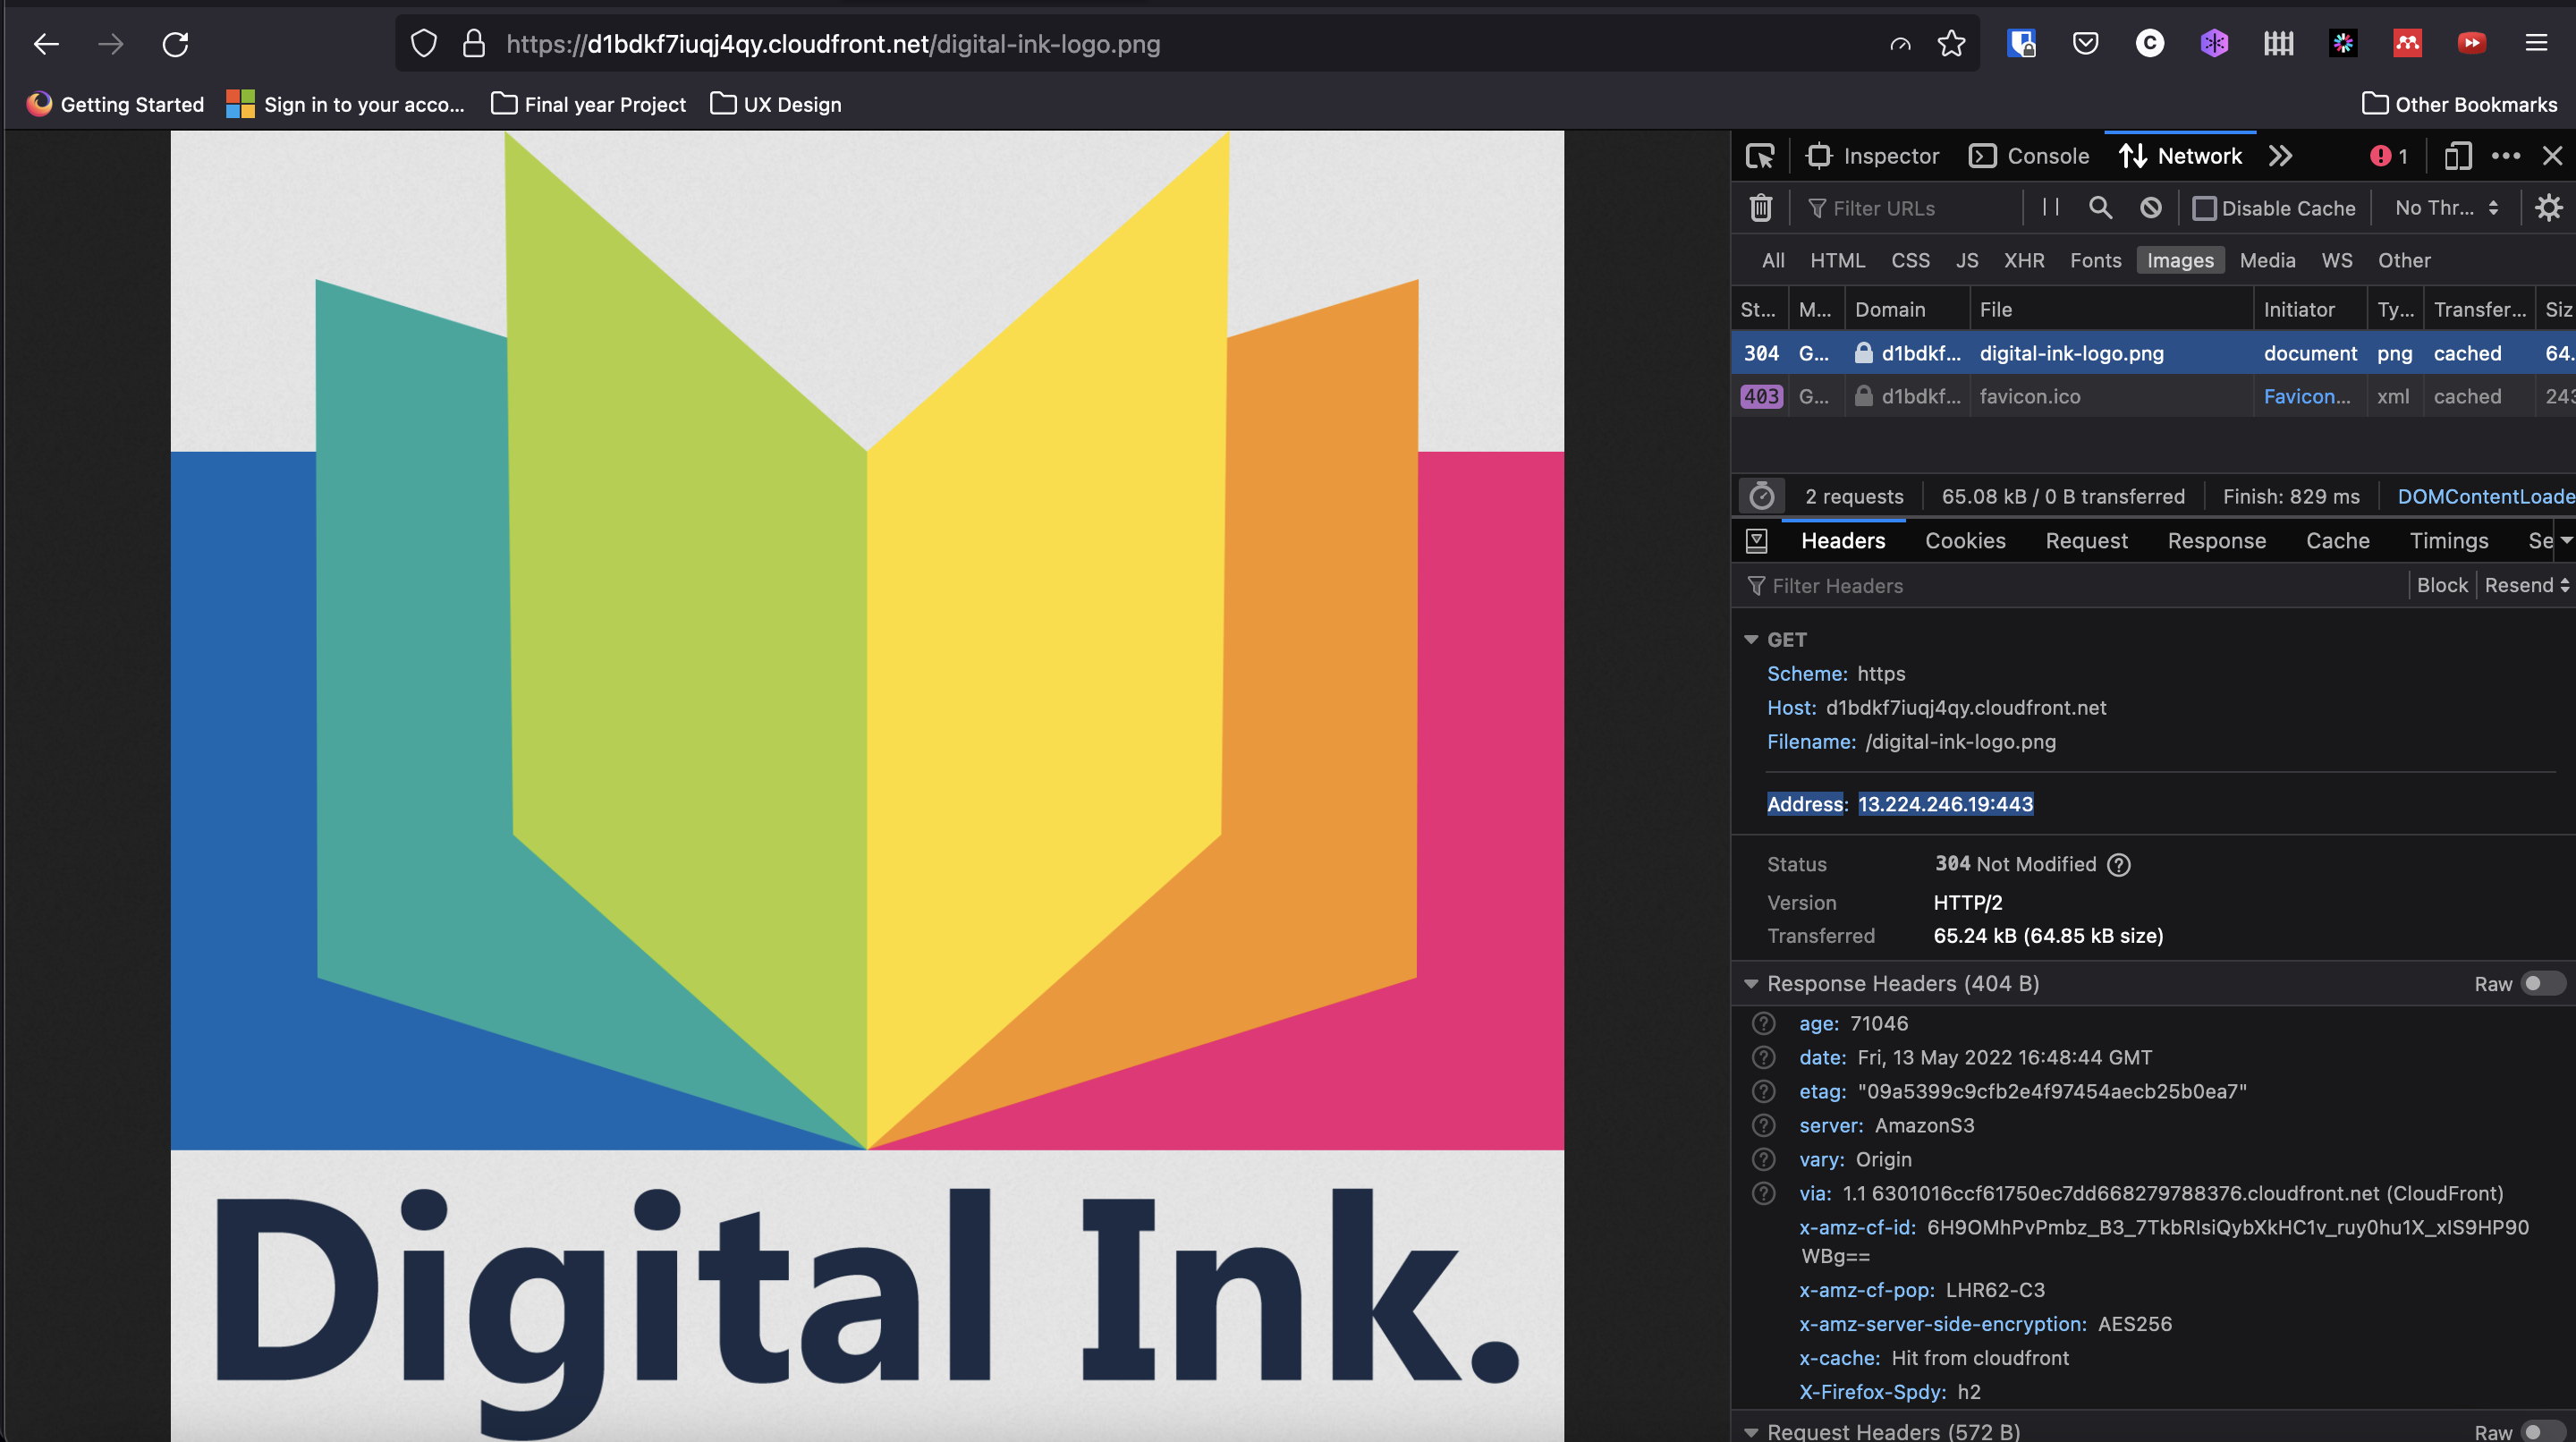
\includegraphics[width=\textwidth]{resources/cloudfront/cloudfront-test-uk}
    \caption{Digital Ink image whilst connected to UK IP.}
    \label{fig:cloudfront-test--uk}
\end{figure}

\begin{figure}[!htbp]
    \centering
    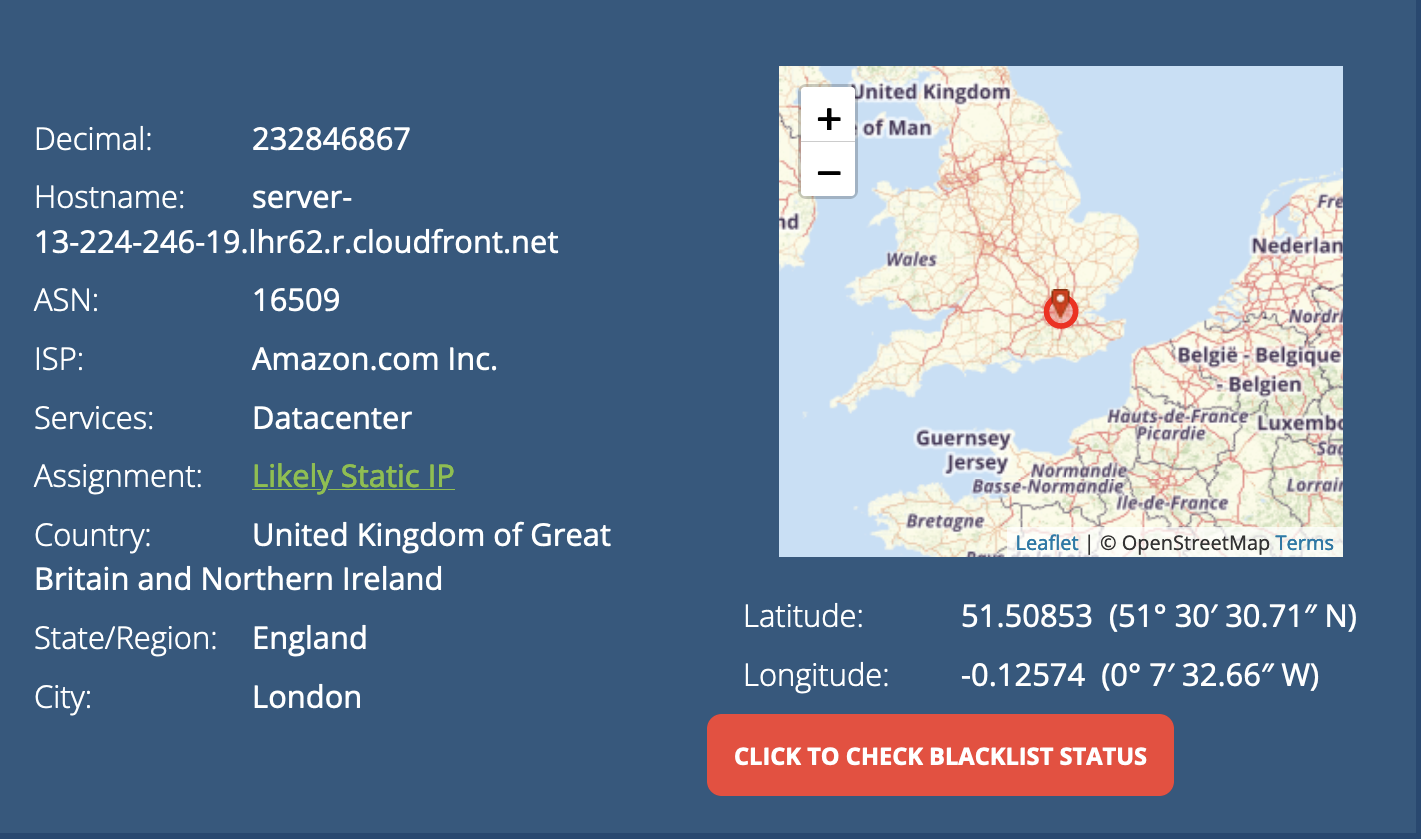
\includegraphics[width=\textwidth]{resources/cloudfront/cloudfront-test-uk-ip}
    \caption{UK IP Location.}
    \label{fig:cloudfront-test-uk-ip}
\end{figure}

\begin{figure}[!htbp]
    \centering
    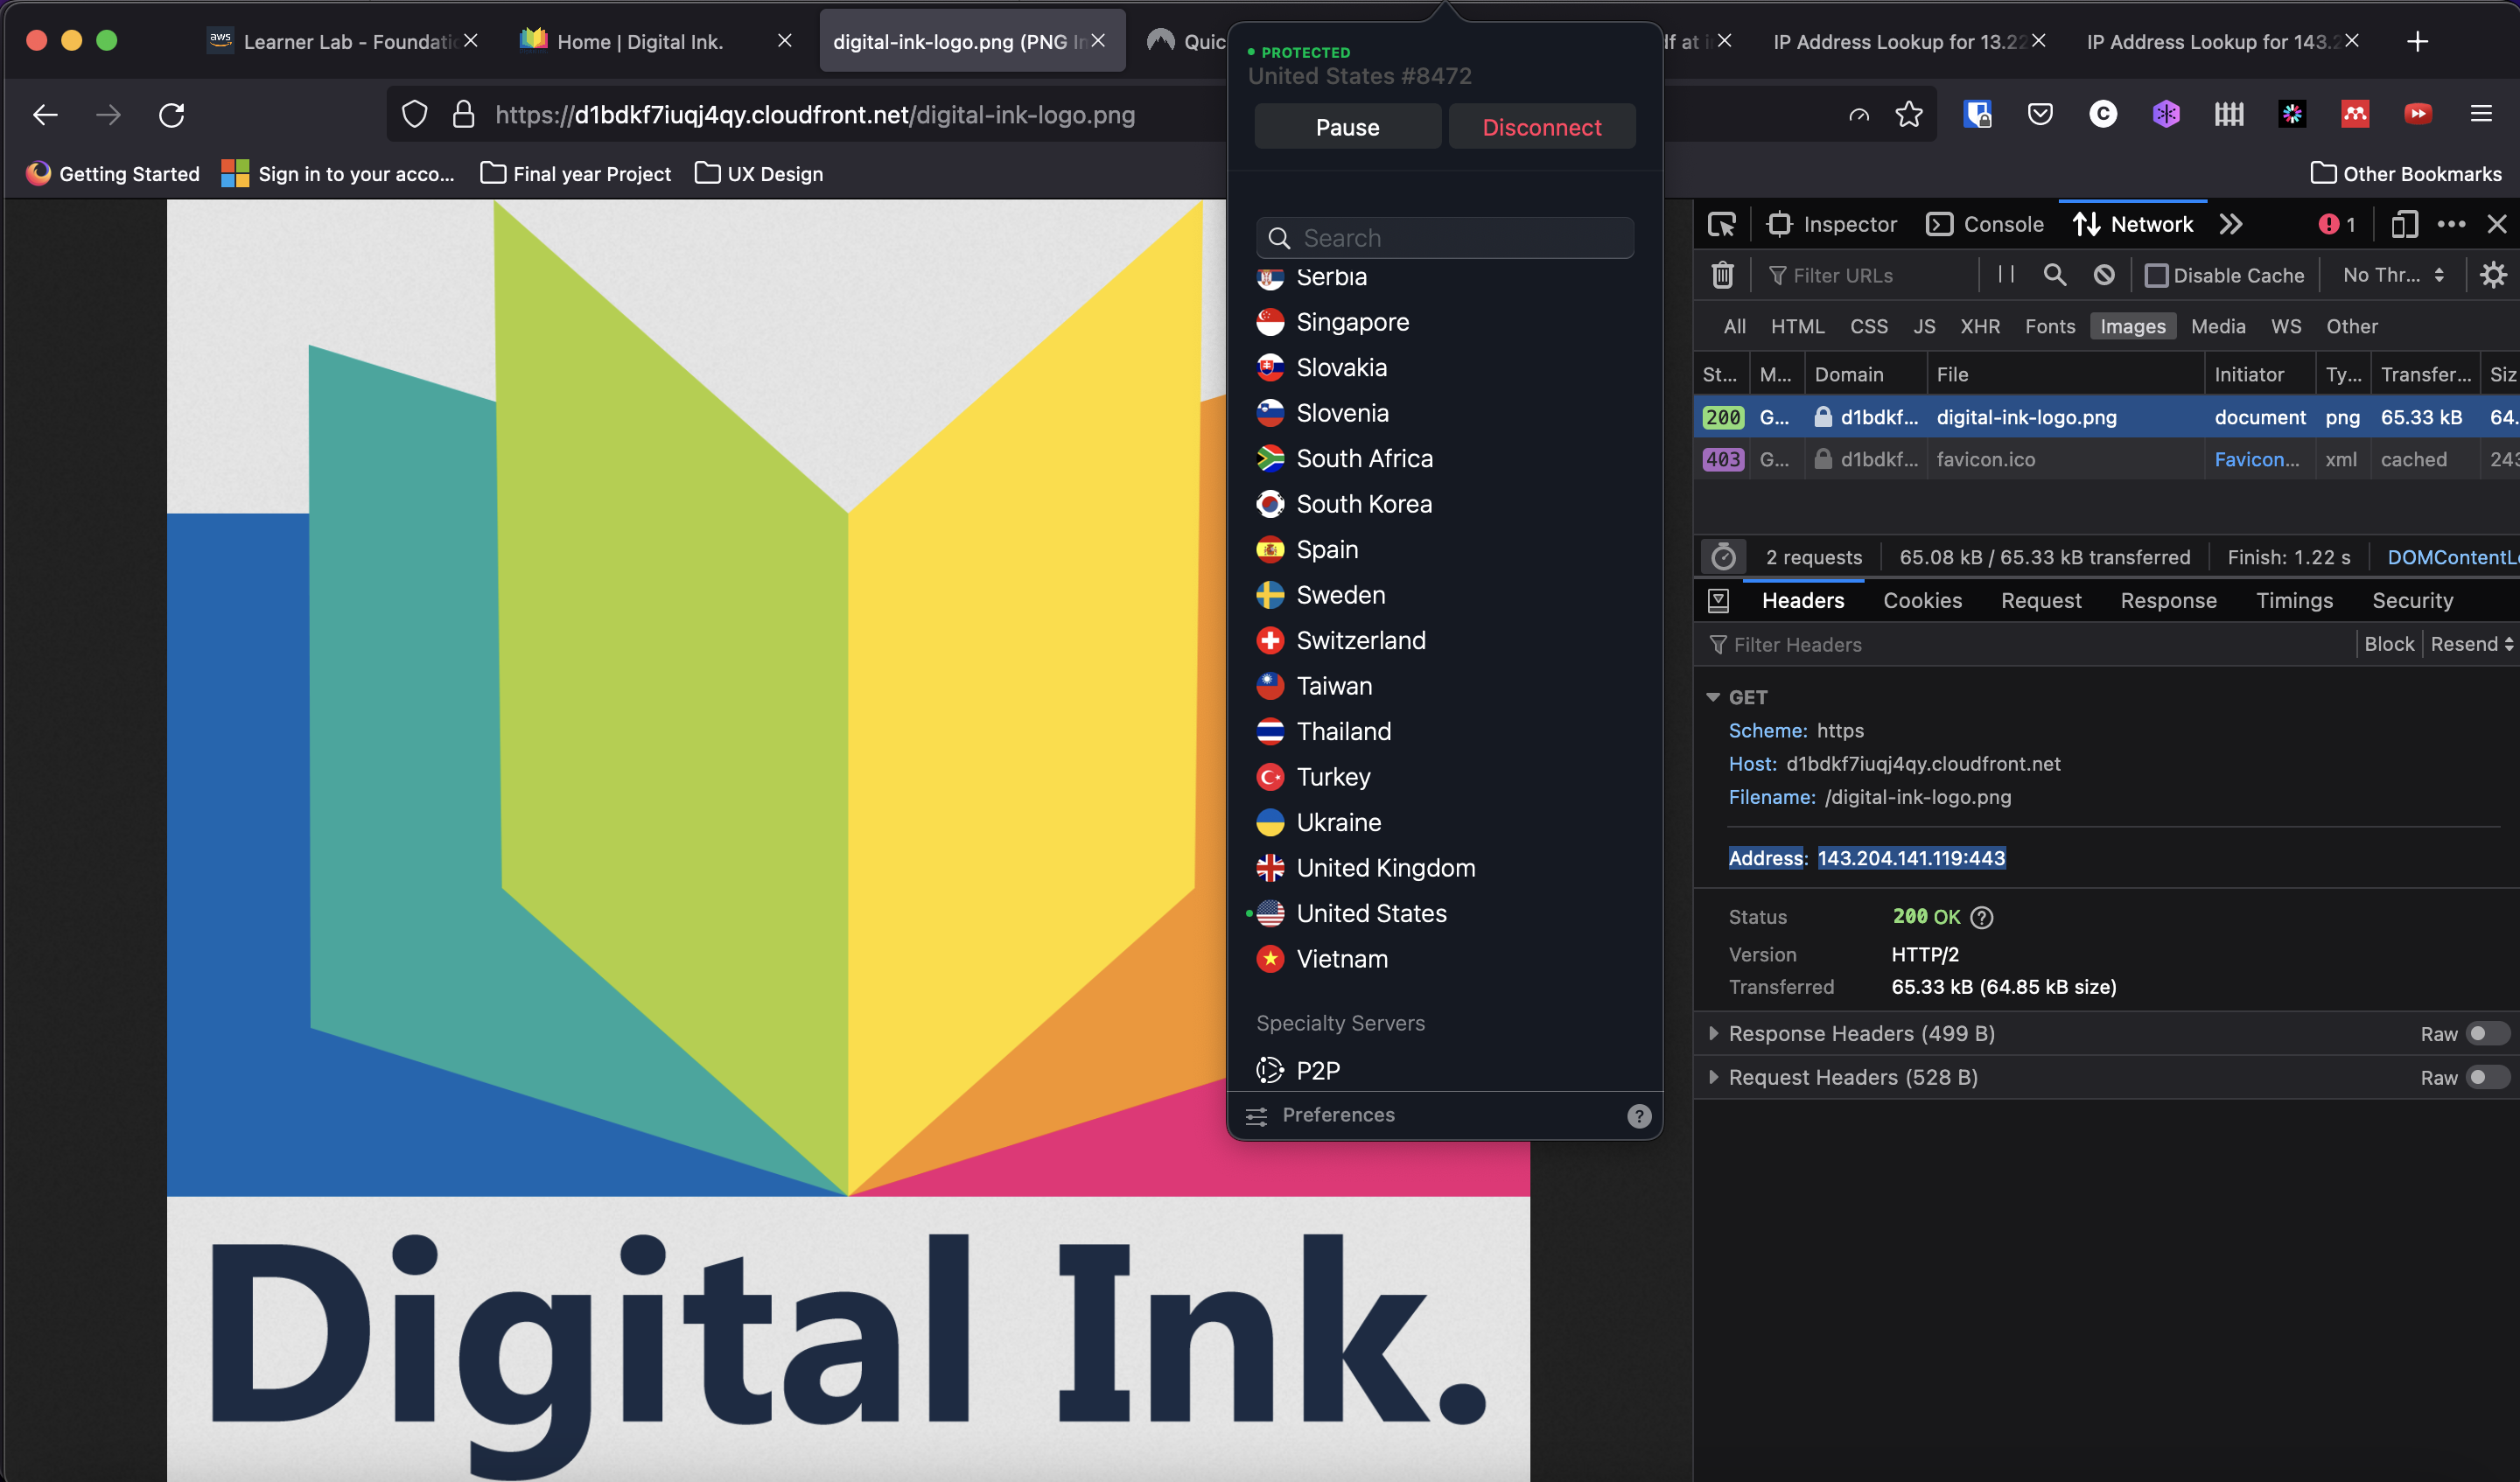
\includegraphics[width=\textwidth]{resources/cloudfront/cloudfront-test-us}
    \caption{Digital Ink image whilst connected to US IP.}
    \label{fig:cloudfront-test-us}
\end{figure}

\begin{figure}[!htbp]
    \centering
    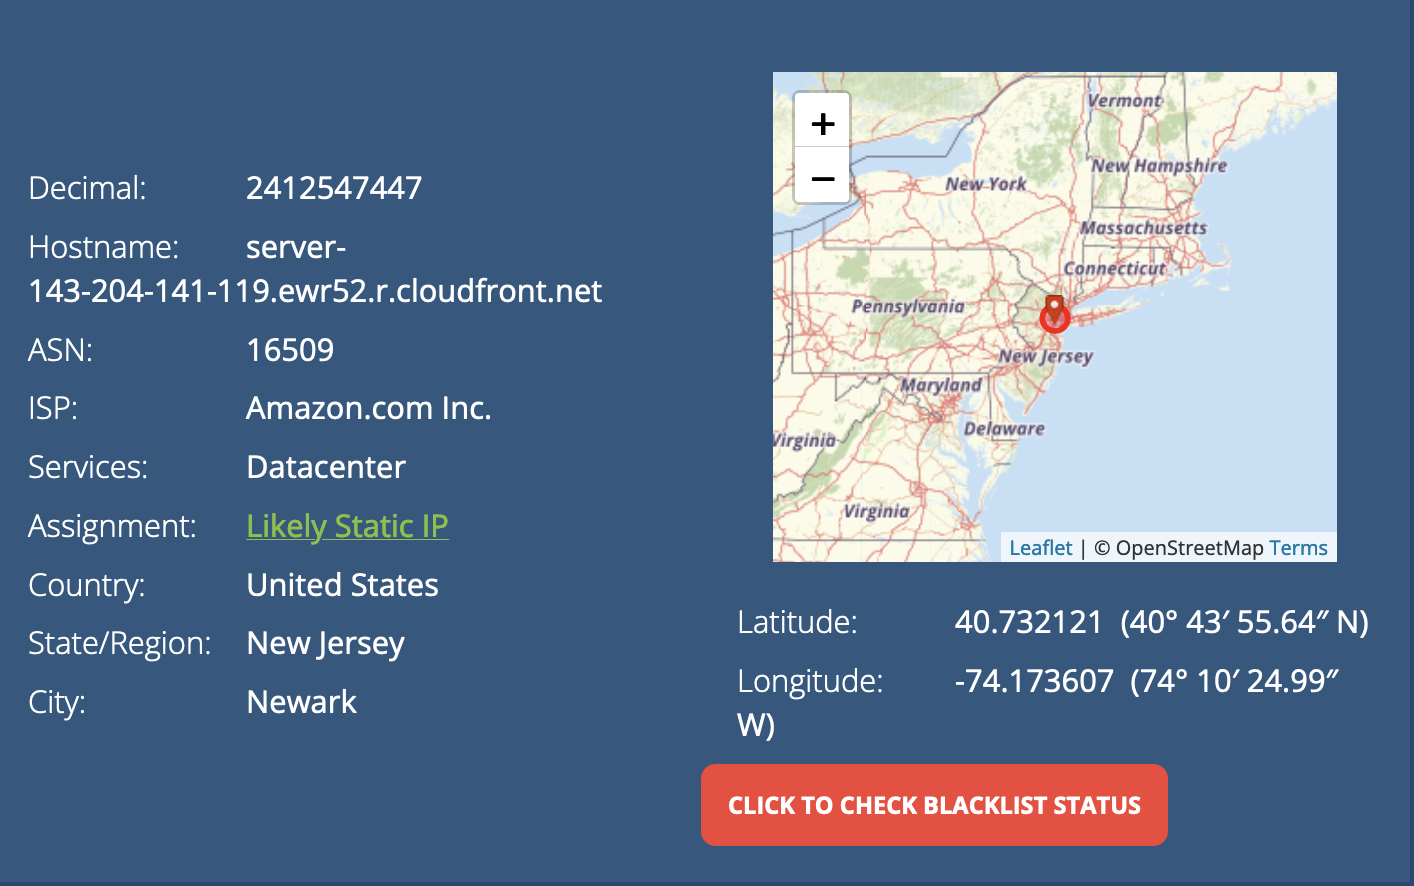
\includegraphics[width=\textwidth]{resources/cloudfront/cloudfront-test-us-ip}
    \caption{US IP Location.}
    \label{fig:cloudfront-test-us-ip}
\end{figure}

\clearpage

\section{Testing RDS}\label{sec:testing-rds}

\begin{figure}[!htbp]
    \centering
    \begin{minted}{cucumber}
Scenario: Creating user information through the web app.
    Given ...
    When ...
    Then ...
    \end{minted}
    \label{fig:create-user-data}
\end{figure}

\begin{figure}[!htbp]
    \centering
    \begin{minted}{cucumber}
Scenario: Creating story information through the web app.
    Given ...
    When ...
    Then ...
    \end{minted}
    \label{fig:create-story-data}
\end{figure}

\begin{figure}[!htbp]
    \centering
    \begin{minted}{cucumber}
Scenario: Reading user information from the database into the web app.
    Given ...
    When ...
    Then ...
    \end{minted}
    \label{fig:read-user-data}
\end{figure}

\begin{figure}[!htbp]
    \centering
    \begin{minted}{cucumber}
Scenario: Reading story information from the database into the web app.
    Given ...
    When ...
    Then ...
    \end{minted}
    \label{fig:read-story-data}
\end{figure}

\begin{figure}[!htbp]
    \centering
    \begin{minted}{cucumber}
Scenario: Updating user information in the database through the web app.
    Given ...
    When ...
    Then ...
    \end{minted}
    \label{fig:update-user-data}
\end{figure}

\begin{figure}[!htbp]
    \centering
    \begin{minted}{cucumber}
Scenario: Updating story information in the database through the web app.
    Given ...
    When ...
    Then ...
    \end{minted}
    \label{fig:update-story-data}
\end{figure}

\begin{figure}[!htbp]
    \centering
    \begin{minted}{cucumber}
Scenario: Deleting user information in the database through the web app.
    Given ...
    When ...
    Then ...
    \end{minted}
    \label{fig:delete-user-data}
\end{figure}

\begin{figure}[!htbp]
    \centering
    \begin{minted}{cucumber}
Scenario: Deleting story information in the database through the web app.
    Given ...
    When ...
    Then ...
    \end{minted}
    \label{fig:delete-story-data}
\end{figure}

\section{Testing CloudWatch}\label{sec:testing-cloudwatch}

(One test for each of the metrics we set up.)

\begin{figure}[!htbp]
    \centering
    \begin{minted}{cucumber}
Scenario:
    Given ...
    When ...
    Then ...
    \end{minted}
    \label{fig:cloudwatch-}
\end{figure}

\section{Testing CloudTrail}\label{sec:testing-cloudtrail}

(One test for each of the metrics we set up.)

\begin{figure}[!htbp]
    \centering
    \begin{minted}{cucumber}
Scenario:
    Given ...
    When ...
    Then ...
    \end{minted}
    \label{fig:cloudtrail-}
\end{figure}

\section{Testing ELB}\label{sec:testing-elb}

(Test for turning off instance 1. Test for turning off instance 2.)